\documentclass[tikz,border=15pt]{standalone}
\usepackage{amsmath, amssymb}
\usetikzlibrary{matrix, positioning, arrows.meta, backgrounds, fit, decorations.pathreplacing}

\newcommand{\F}{\mathbb{F}}
\newcommand{\ideal}[1]{\langle #1 \rangle}

\begin{document}
	
	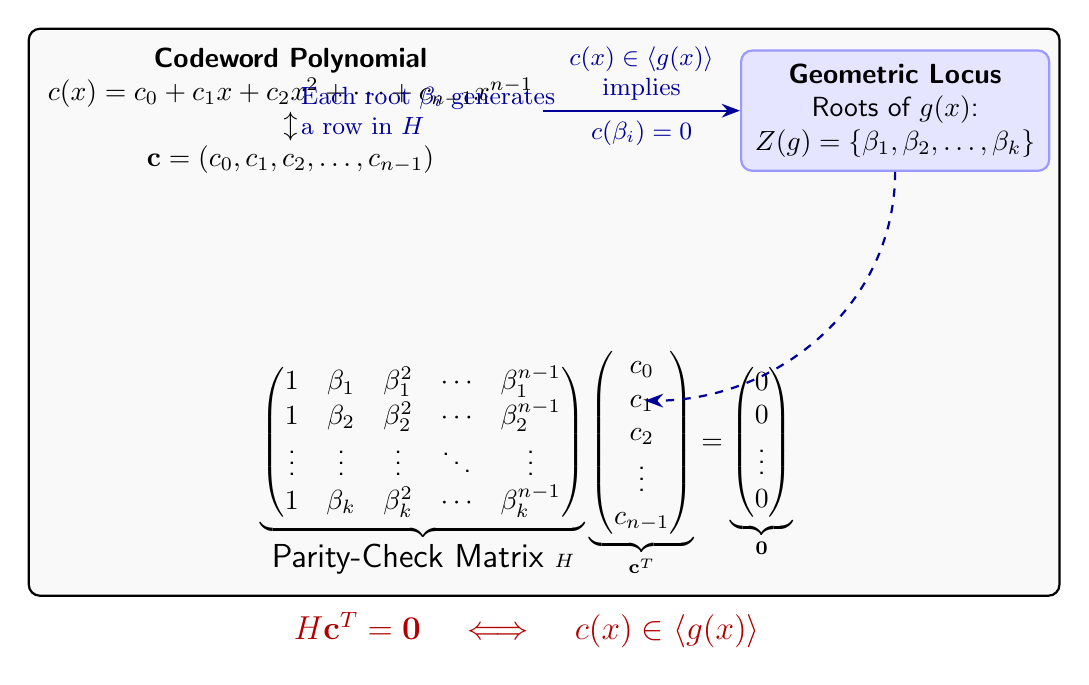
\begin{tikzpicture}[
		>=Stealth,
		node distance=1.5cm,
		font=\sffamily,
		highlight/.style={fill=blue!10, rounded corners, inner sep=5pt}
		]
		
		% ==========================================
		% STEP 1: The Code Vector
		% ==========================================
		\node (codeword) [align=center] {
			\textbf{Codeword Polynomial} \\
			$c(x) = c_0 + c_1x + c_2x^2 + \dots + c_{n-1}x^{n-1}$ \\
			$\updownarrow$ \\
			$\mathbf{c} = (c_0, c_1, c_2, \dots, c_{n-1})$
		};
		
		% ==========================================
		% STEP 2: The Roots (Geometry)
		% ==========================================
		\node (roots) [highlight, right=2.5cm of codeword, align=center, draw=blue!40, thick] {
			\textbf{Geometric Locus} \\
			Roots of $g(x)$: \\
			$Z(g) = \{\beta_1, \beta_2, \dots, \beta_k\}$
		};
		
		\draw[->, thick, blue!60!black] (codeword) -- (roots) 
		node[midway, above, align=center, font=\small] {$c(x) \in \ideal{g(x)}$ \\ implies}
		node[midway, below, align=center, font=\small] {$c(\beta_i) = 0$};
		
		% ==========================================
		% STEP 3: The Matrix Construction
		% ==========================================
		\node (matrix_eq) [below=2cm of codeword, xshift=3cm] {
			$\underbrace{
				\begin{pmatrix}
					1 & \beta_1 & \beta_1^2 & \cdots & \beta_1^{n-1} \\
					1 & \beta_2 & \beta_2^2 & \cdots & \beta_2^{n-1} \\
					\vdots & \vdots & \vdots & \ddots & \vdots \\
					1 & \beta_k & \beta_k^2 & \cdots & \beta_k^{n-1}
				\end{pmatrix}
			}_{\text{\large Parity-Check Matrix } H}
			\underbrace{
				\begin{pmatrix}
					c_0 \\ c_1 \\ c_2 \\ \vdots \\ c_{n-1}
				\end{pmatrix}
			}_{\mathbf{c}^T}
			=
			\underbrace{
				\begin{pmatrix}
					0 \\ 0 \\ \vdots \\ 0
				\end{pmatrix}
			}_{\mathbf{0}}$
		};
		
		% Arrows pointing from roots to rows
		\draw[->, thick, dashed, blue!60!black] 
		(roots.south) to[out=270, in=0] ([yshift=0.8cm, xshift=1.5cm]matrix_eq.center)
		node[pos=0.4, right, align=left, font=\small] {Each root $\beta_i$ generates \\ a row in $H$};
		
		% Annotations
		\node[below=0.2cm of matrix_eq, font=\large\bfseries, color=red!70!black] {
			$H \mathbf{c}^T = \mathbf{0} \quad \Longleftrightarrow \quad c(x) \in \ideal{g(x)}$
		};
		
		% Structural Box
		\begin{scope}[on background layer]
			\node[draw, thick, fill=gray!5, rounded corners, fit=(codeword)(roots)(matrix_eq)] {};
		\end{scope}
		
	\end{tikzpicture}
	
\end{document}